\documentclass{article}
\usepackage[T1]{fontenc}
\usepackage{lmodern}
\usepackage{graphicx}
\usepackage{amsmath,amssymb}
\usepackage[a4paper,margin=2cm]{geometry}
\usepackage[absolute,overlay]{textpos}
\setlength{\TPHorizModule}{1mm}
\setlength{\TPVertModule}{1mm}
\usepackage[indonesian]{babel}
\usepackage{hyperref}
\setlength{\emergencystretch}{2em}
% unit: Halaman 5

\begin{document}

% === Halaman 5 (llm) ===

\section*{Bit, Byte, dan Kode Heksadesimal}

\vspace{68.31mm}

\begin{itemize}
    \item Pesan di dalam \textit{cipher} modern dienkripsi bit-per-bit atau \textit{byte-per-byte}, atau dalam kelompok bit (\textit{byte}).
    \[ 1\text{ byte} = 8\text{ bit} \]
    \item Pada beberapa algoritma kriptografi, pesan dikodekan ke dalam kode heksadesimal (\textbf{Hex}).
    \[ 1\text{ kode hex} = 4\text{ bit} \]
    \vspace{5mm}
    \item Contoh: Pesan $\text{1001110101101010}$ dalam kode Hex dengan cara membagi pesan menjadi blok 4-bit:
    \[ \text{1001 1101 0110 1010 = 9D6A} \]
\end{itemize}

% deskripsi: Tabel konversi biner 4-bit ke kode heksadesimal
% bbox normalisasi: [0.1300, 0.4800, 0.6700, 0.7100]
\begin{textblock*}{113.40mm}(27.30mm,142.56mm)
\noindent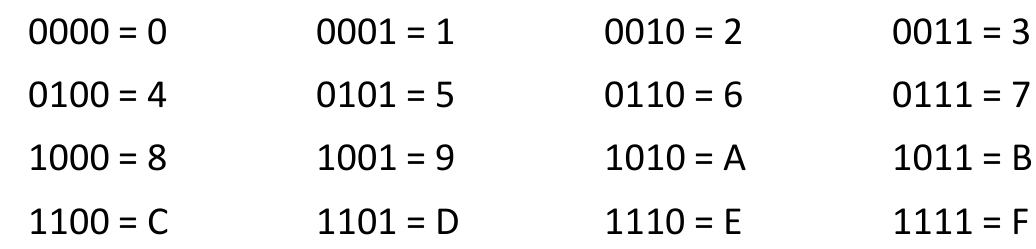
\includegraphics[width=113.40mm,height=68.31mm]{../../images/llm/page_005_img_01.png}%
\end{textblock*}

\end{document}
